\documentclass{sig-alternate-sigmod09}

\usepackage[bookmarks=true,pdfborder= 0 0 0]{hyperref}

\usepackage{tikz}
\usetikzlibrary{calc,trees,positioning,arrows,chains,shapes.geometric,%
  decorations.pathreplacing,decorations.pathmorphing,shapes,%
  matrix,shapes.symbols,plotmarks,decorations.markings,shadows}

\DeclareMathOperator{\atantwo}{atan2}

\hypersetup{
pdfauthor={Patrick Brosi},
pdfkeywords=,
pdftitle={Metro Maps on Octilinear Grid Graphs},
pdfsubject={},
pdfcreator={},
pdfproducer={}
}

\newcommand\todo[1]{\textcolor{blue}{[TODO: #1]}}
\newcommand\TODO[1]{\textcolor{blue}{\small [TODO: #1]}}

\begin{document}
\title{Metro Maps on Octilinear Grid Graphs}

\numberofauthors{1}
%\author{Patrick Brosi\\\affaddr{University of Freiburg}\\\affaddr{Chair of Algorithms and Data Structures}}

\maketitle

\section{Abstract}

We investigate a novel approach to the problem of drawing octilinear Metro Maps.
We state the problem as a batch of shortest-path calculations on a specially crafted octilinear grid graph, where edge bends are implicitely added to the cost metric.
Our approach can be optimized exactly via an Integer Linear Program (ILP) or approximately by iteratively calculating shortest-paths between node candidates in the octilinear grid graph.
Most importantly, our approach allows us to revisit earlier work [Stott] which used local search techniques to update the node positions until a (local) optimum was found, but where octilinearity was not guaranteed.
By recalculating the shortest-path between an updated node and its neighbors on our octilinear grid graph, we can guarantee octilinearity.
Using this approach, we can calculate maps which are nearly optimal in a fraction of a second for medium-sized networks.
As far as we are aware, our technique is the first non-global approach which guarantees octilinear results, albeit at the cost of not always finding a solution. The resulting schematic maps are rendered using previous work and are publicly accessible.

\section{Introduction}


\TODO{Write intro}

\begin{figure*}[t]
  \centering
	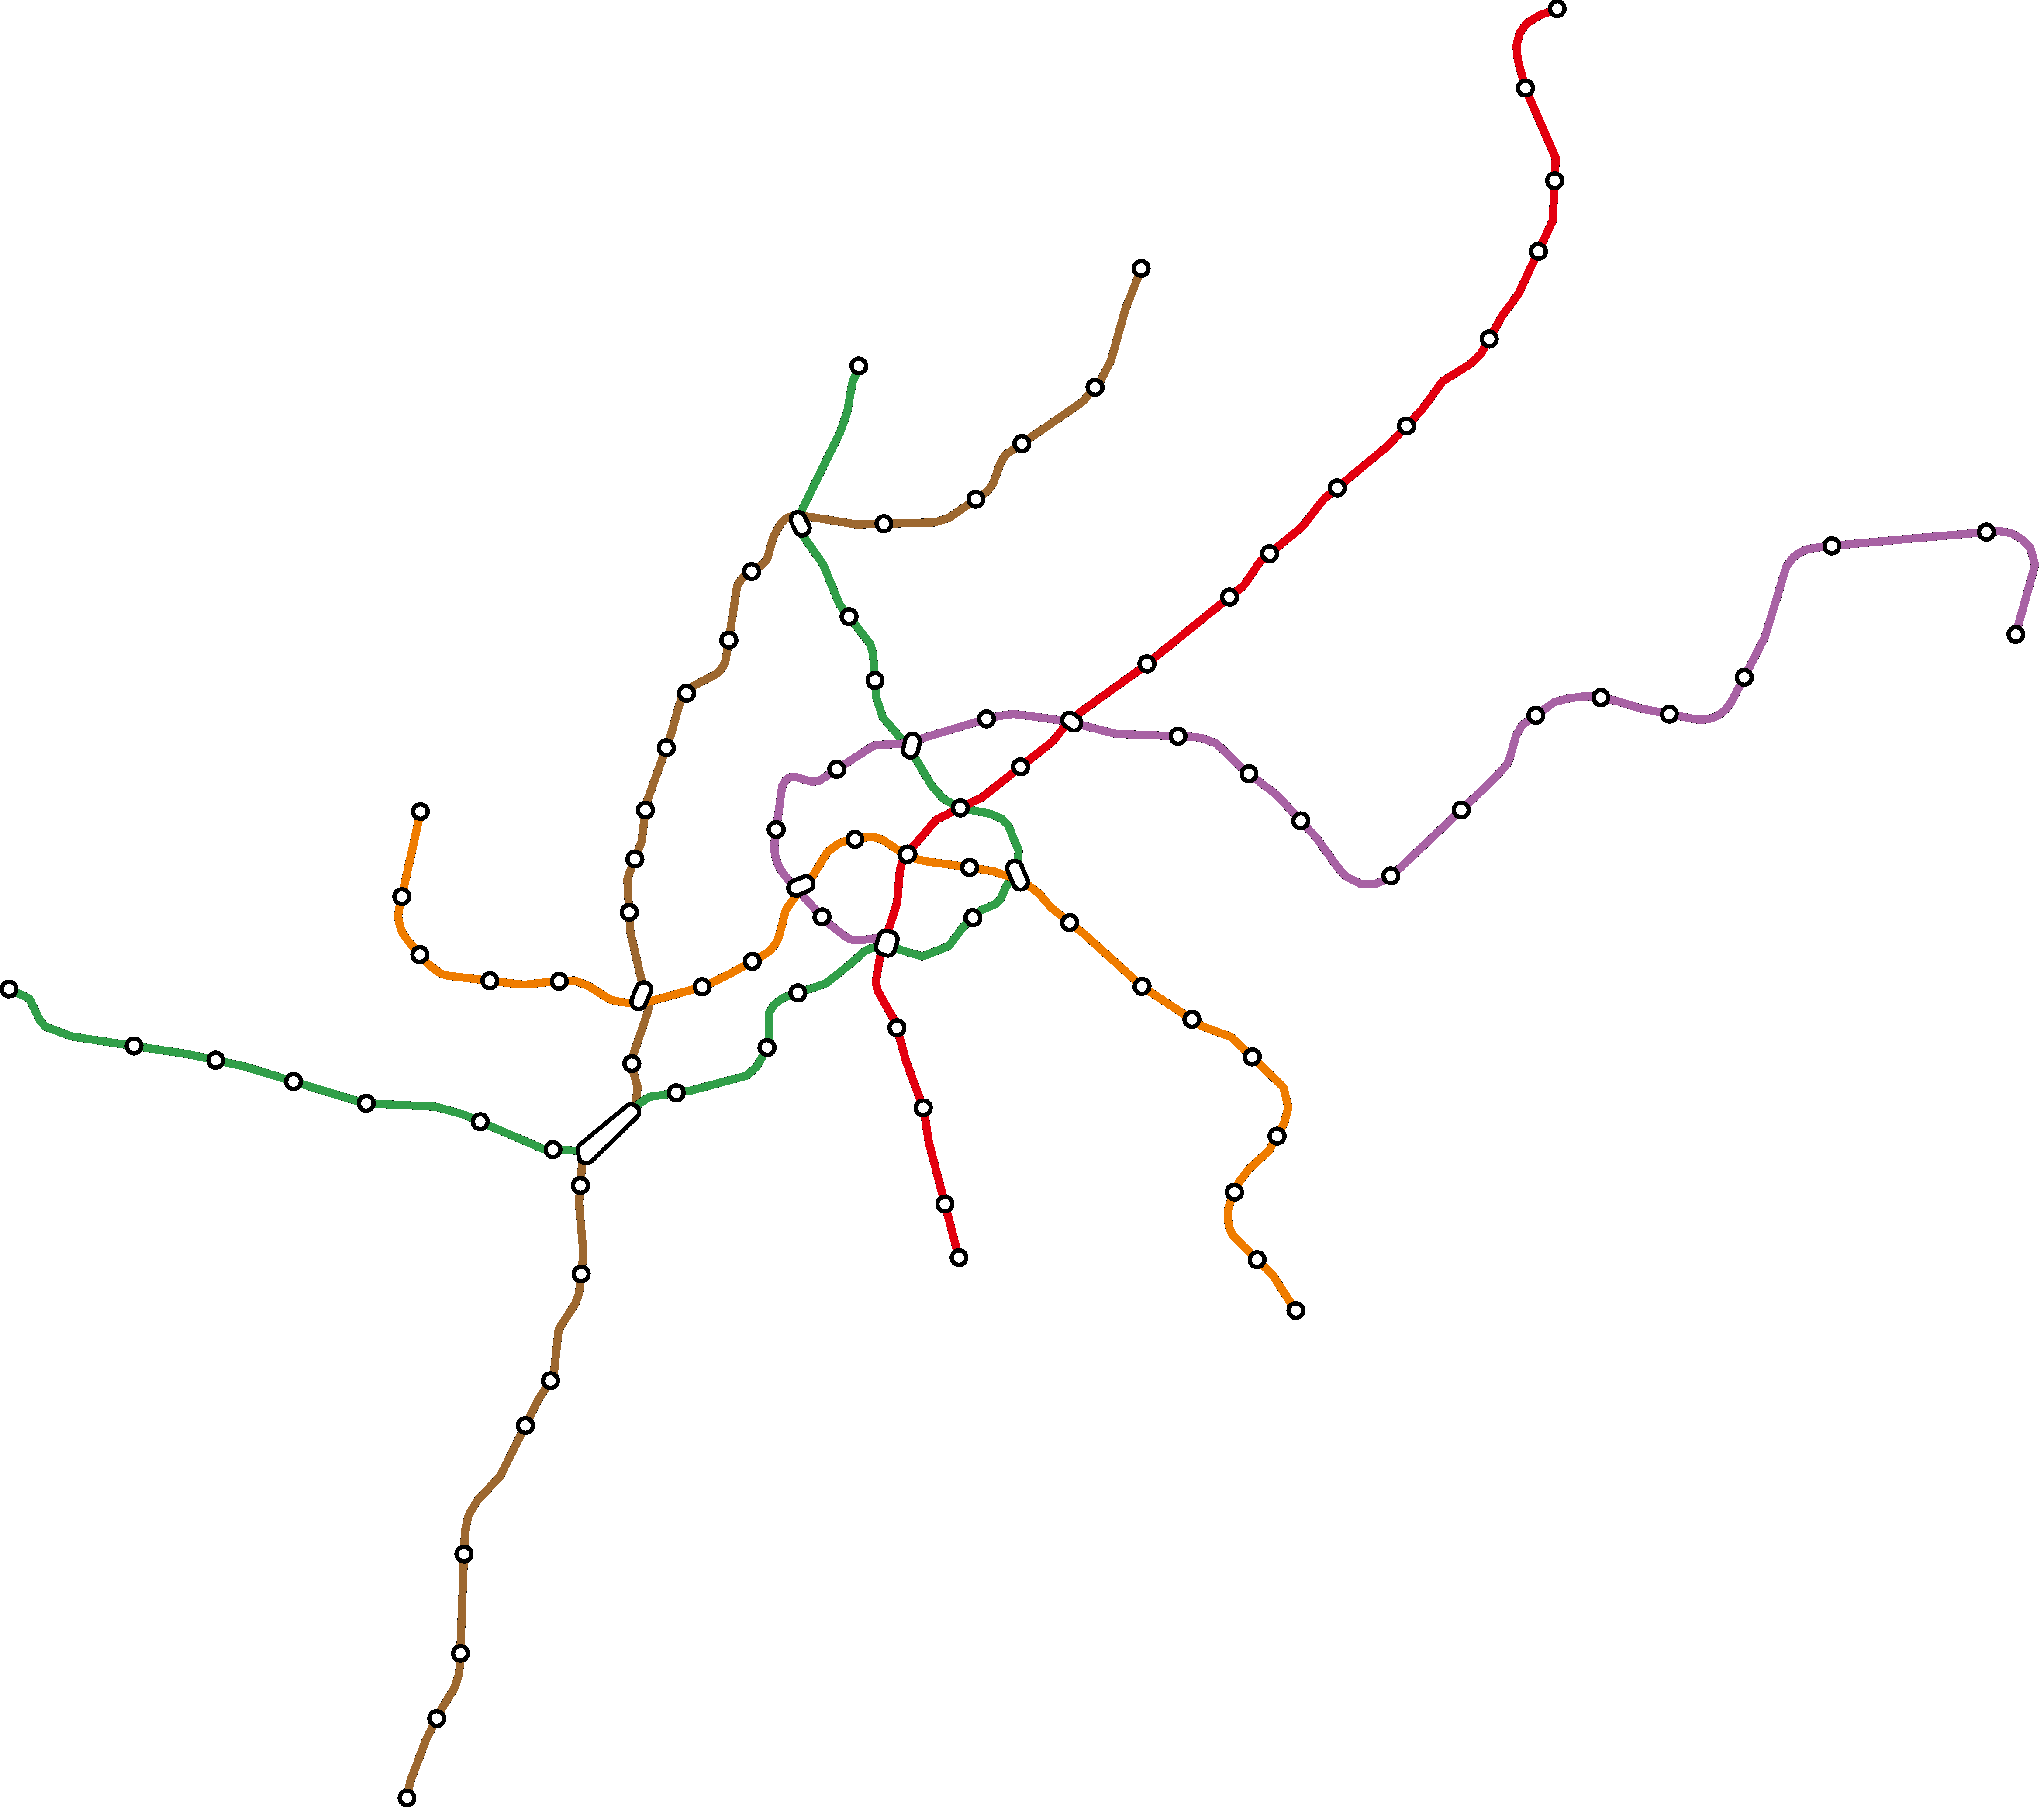
\includegraphics[width=0.474\textwidth]{figures/octi_input.pdf}
	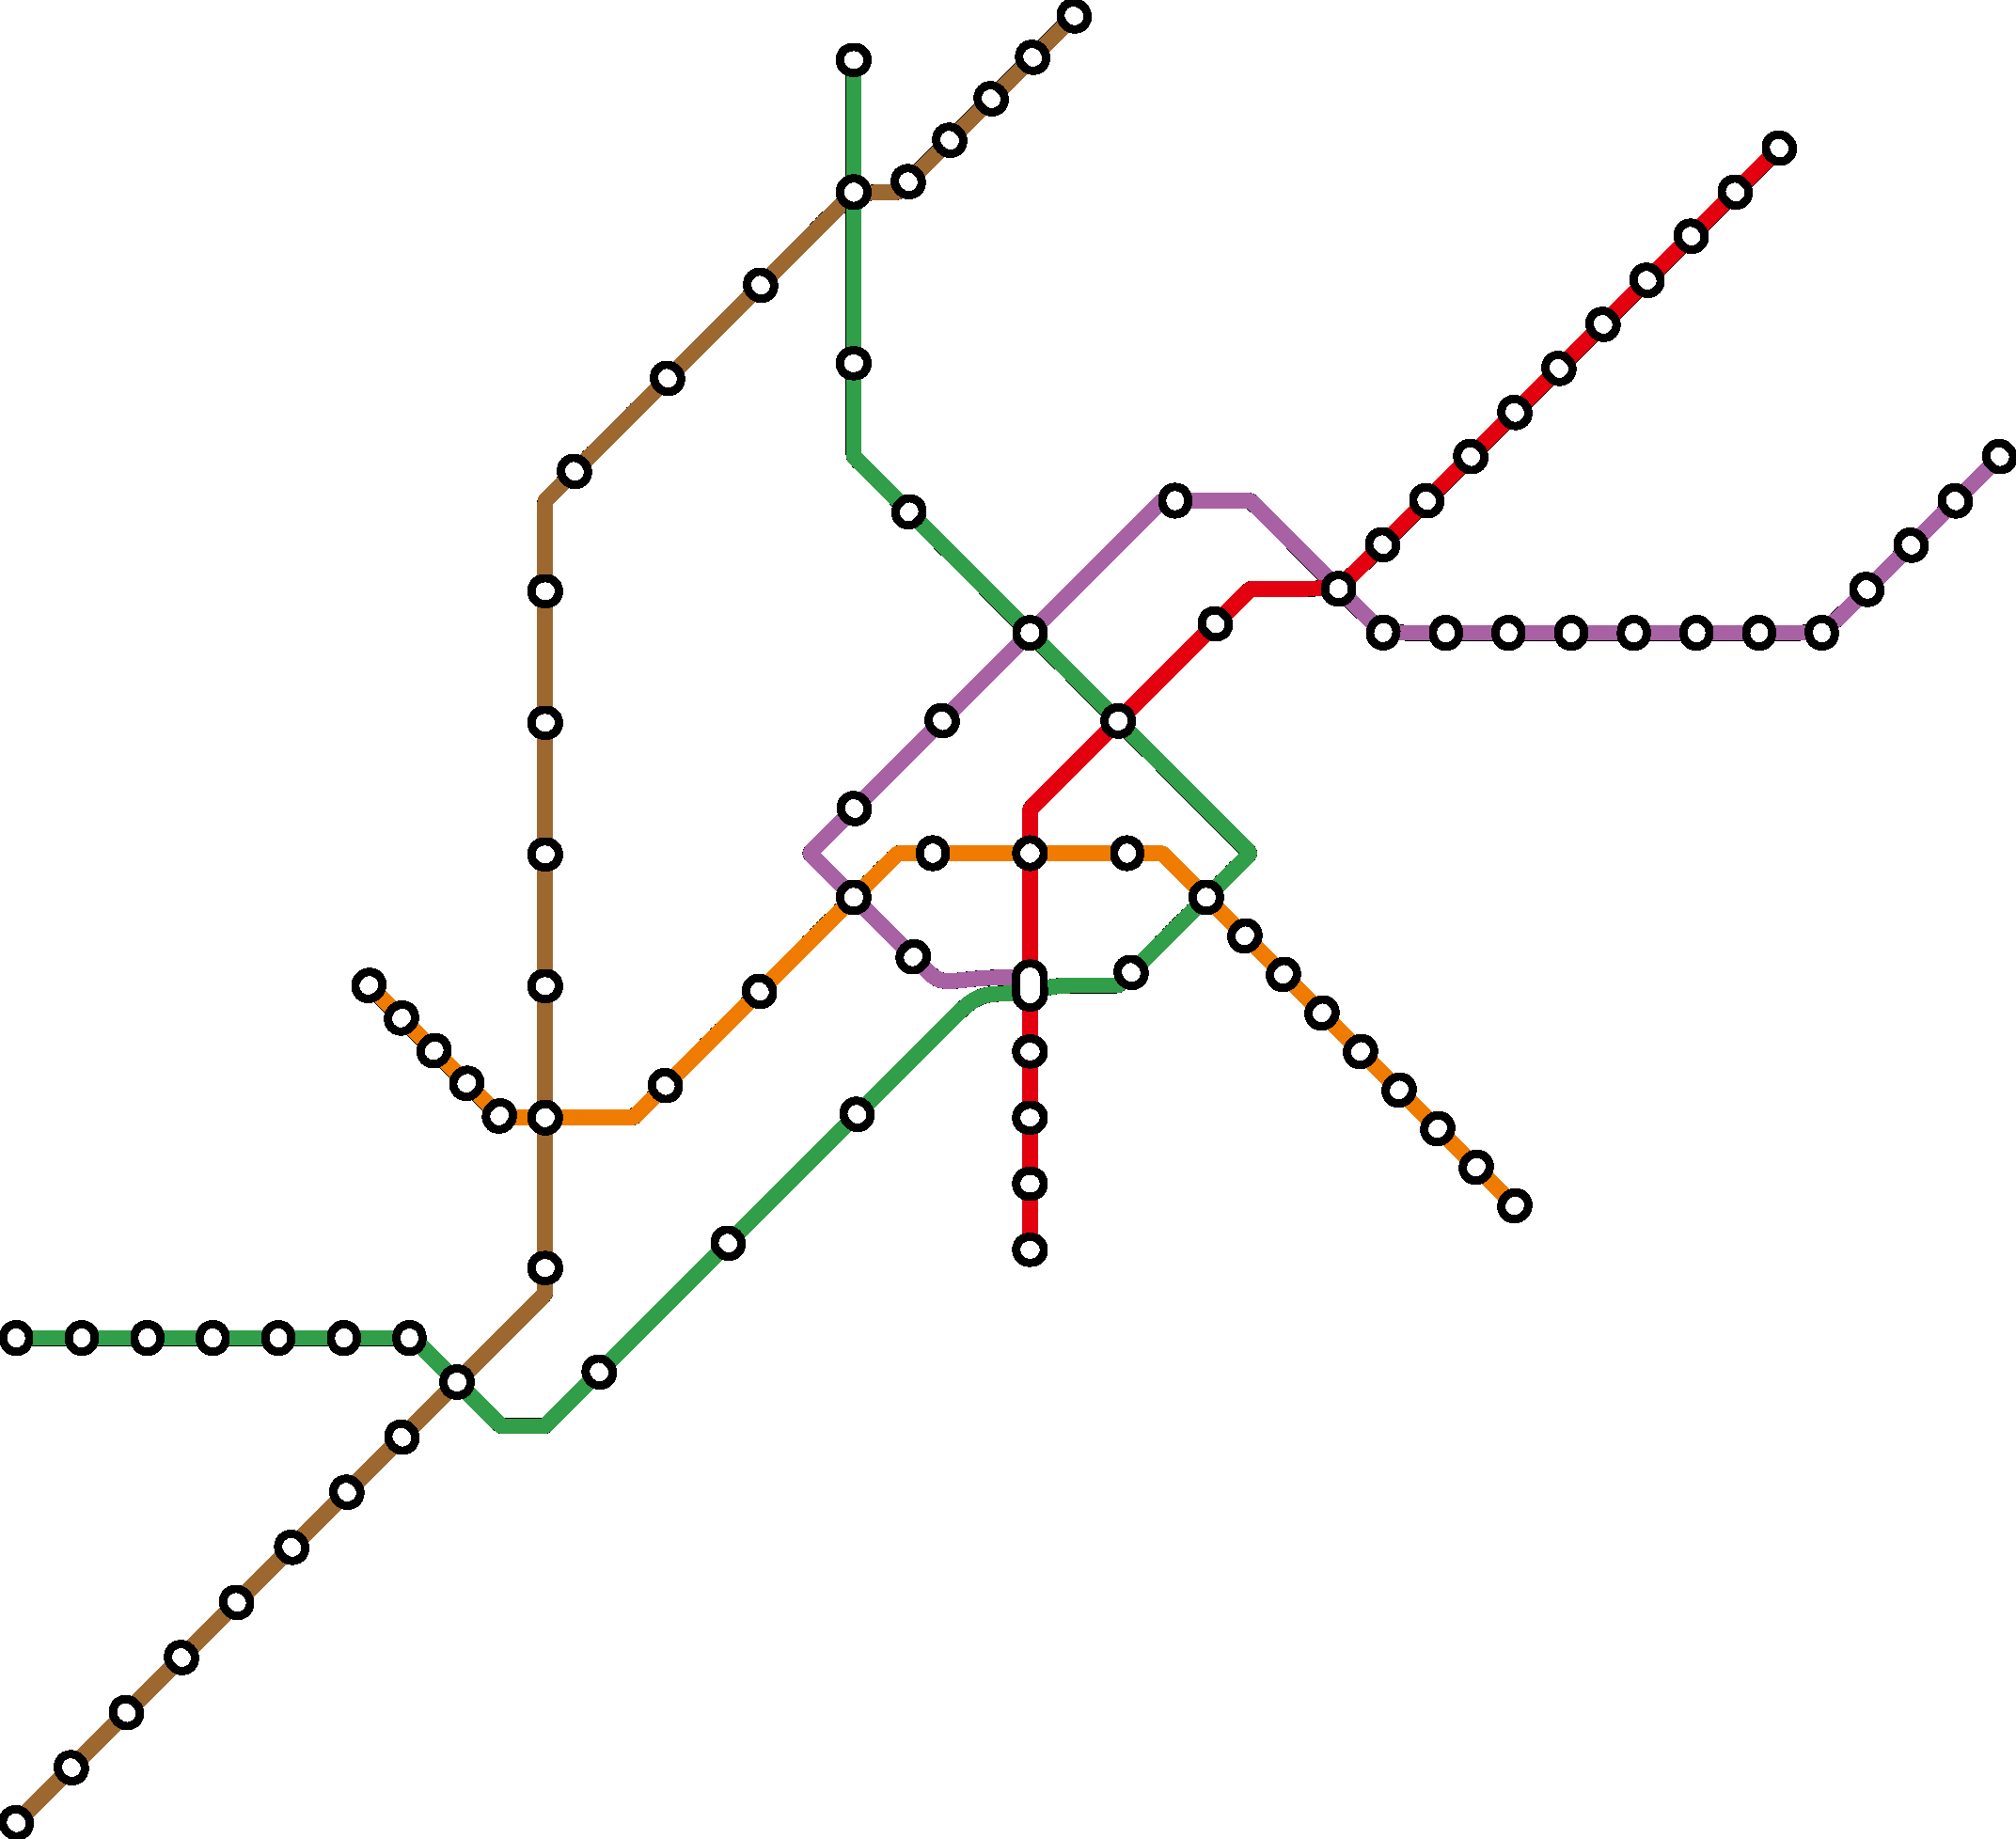
\includegraphics[width=0.474\textwidth]{figures/octi.pdf}
	\caption{The subway network of Vienna, rendered with our approach from raw timetable (GTFS) data (including stop positions).}
	\label{FIG:examplewien}
\end{figure*}

\section{Problem definition}

Given an undirected planar graph $G = \{V, E\}$. We say $\mathcal{D}_G = \{p, c\}$ is a drawing of $G$, where $p(v) \in \mathbb{R}^2$ assigns a position to every node $v \in V$ and $c(e) = (q_0, q_1, ..., q_n)$, $q_i \in \mathbb{R}^2$ assigns a piecewise linear curve to every edge $e \in E$. The initial input drawing $\mathcal{D}_G$ assigns each node a geographical real-world position, and each edge an (optional) real-world trajectory.
Our goal is to find a schematic drawing $\mathcal{D}'_G$ that resembles a classic Metro Map.
This is usually formalized as a set of hard and soft constraints \cite{nb, ...}.
The hard constraints may be summarized as:
\begin{enumerate}
\setlength\itemsep{.1em}
\item \emph{Octilinearity}. Each edge curve $c(e)$ may only consist of segments whose orientation is a multiple of $45^{\circ}$.
\item \emph{Topology preservation}. The input embedding should be respected. In particular, no crossings between edges should be introduced and non-incident edges should never share common points. This is often modelled as a minimum distance $d_{e}$ between non-incident edge curves and a minimum distance $d_{v}$ between node positions.
\end{enumerate}
Additionally, the following soft constraints are usually employed:
\begin{enumerate}
\setlength\itemsep{.1em}
\item \emph{Edge monotony}. Minimize the number of turns an edge has to take. Prefer large angles.
\item \emph{Geographical accuracy}. The original node positions should be changed as little as possible.
\item \emph{Map density}. \TODO{describe that we want to minimize edge lengths}
\end{enumerate}

With respect to edge monotony and octilineary, previous work often stated the problem as finding an octilinear embedding of the input graph, where each edge is represented by a straight octilinear arc.


\section{Related Work}

Survey Nöllenburg %http://i11www.iti.kit.edu/extra/publications/n-asamm-14.pdf
Survey Wolff %http://www1.pub.informatik.uni-wuerzburg.de/pub/wolff/pub/w-dsms-07.pdf
Hong et al., force-based approach
Stott's PhD
steiner trees! %https://www.researchgate.net/profile/Matthias_Mueller-Hannemann/publication/225160153_Approximation_of_Octilinear_Steiner_Trees_Constrained_by_Hard_and_Soft_Obstacles/links/0912f50cf248ec1193000000/Approximation-of-Octilinear-Steiner-Trees-Constrained-by-Hard-and-Soft-Obstacles.pdf

\section{Octilinear Grid Graph}

We use an auxiliary undirected graph $\Omega = \{V_\omega, E_\omega\}$ on which every possible path $(v_0, v_1, ..., v_n), v_i \in V_\Omega$ represents an octilinear curve. The graph in Fig.~\ref{FIG:gridgraph} trivially satisfies this: we define a $x\times y$ grid and add nodes $v_{x,y}$ to $V_\omega$ for every grid point.
Each node $v_{x,y}$ is connected with its 8 direct neighbors (except at the grid boundaries) $n^0(v_{x,y}) ... N^7(v_{x, y})$, where $N^0(v_{x, y})$ is the ``north'' neighbor of $v_{n, m}$,  $N^1(v_{x, y})$ the ``north-east'' neighbor and so on, in clockwise fashion.

To later be able to optimize soft constraint (1), we additionally want the total cost for a path in $\Omega$ to reflect the number and accuteness of turns.
The penalty for a turn should be weighted by its degree - either $135^{\circ}$, $90^{\circ}$ or $45^{\circ}$.
We call these penalties $p_{135}$, $p_{90}$ and $p_{45}$.
A straight pass through a node should go unpunished, that is, $p_{180} = 0$.
Since we aim for a ``smooth'' path through $G$ and want to favor obtuse angles, we require $p_{180} < p_{135} < p_{90} < p_{45}$.

\TODO{mention cost sum of a path, derive the constant a below from it}

\begin{figure}
  \centering
	$\vcenter{\hbox{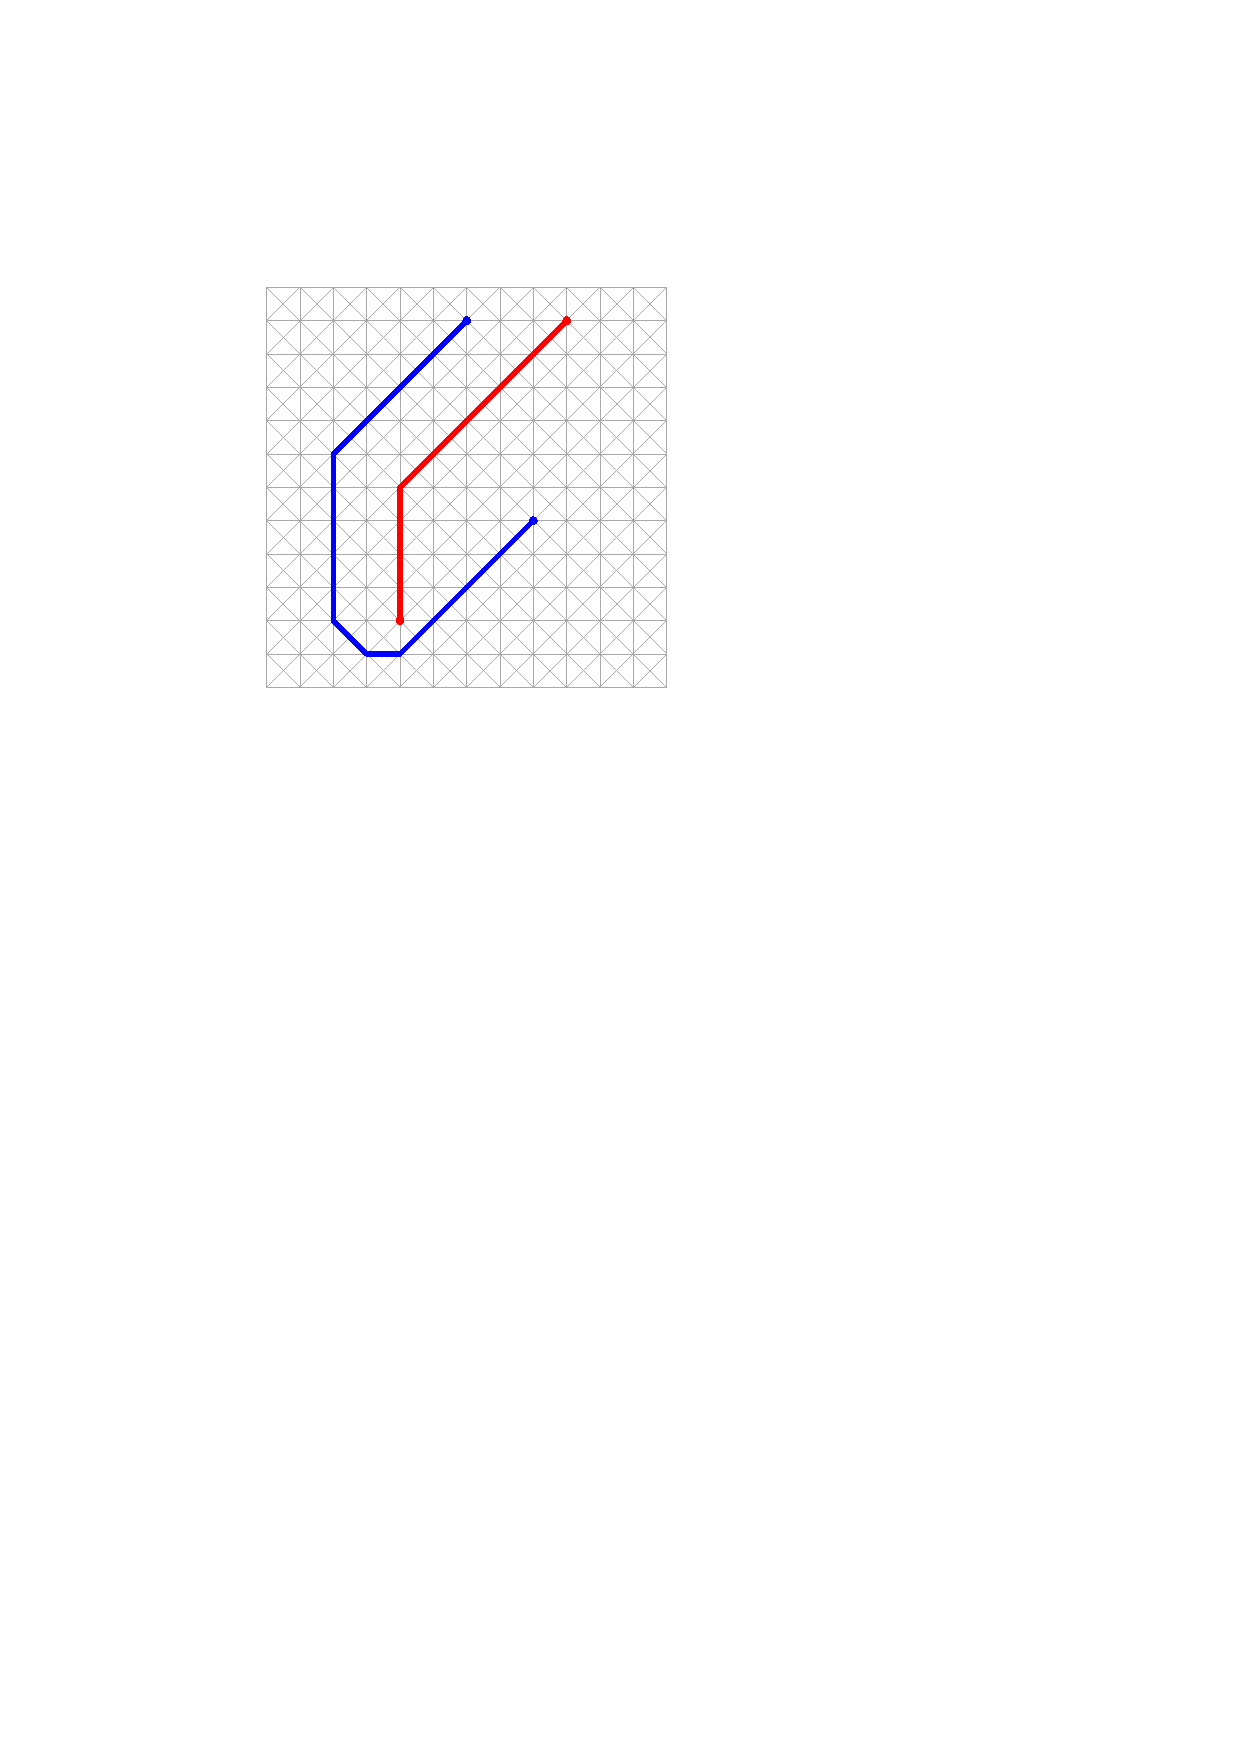
\includegraphics[width=0.474\textwidth]{figures/grid.pdf}}}$
	\caption{Left: A shortest path between $t$ and $u$ on a grid graph with uniform edge cost. Path turns are not minimized. Right: Two shortest path between $(t, u)$, and $(v, w)$ on our octilinear grid graph with uniform grid edge cost $1$ and additional path turn penalties $p_{135} = 1$, $p_{90} = 3$ and $p_{45} = 9$. Path $(t, u)$ acts as an obstacle for $(v, w)$.}
	\label{FIG:grids}
\end{figure}

We model this by adding 8 auxiliary port nodes $v_{x,y}^{0} ... v_{x,y}^{7}$ to every grid node $v_{x,y}$.
Each port again corresponds to an outgoing angle in clockwise fashion and is connected to $v_{x, y}$ via sink edges $e_{x,y}^0 ... e_{x,y}^7$.
These sink edges allow us to arrive at the original node $v_{x, y}$.
For paths passing through $v_{x, y}$, we connect each port $v_{x, y}^i$ with its 7 sibling ports at $45^{\circ}$, $90^{\circ}$ $135^{\circ}$, $180^{\circ}$, $225^{\circ}$, $270^{\circ}$ and $315^{\circ}$.

As both a $45^{\circ}$ port edge and a $90^{\circ}$ port edge may be substituted by two (or more) cheaper edges, special care has to be applied to the modelling of the actual edge costs.
For example, a $45^{\circ}$ turn can be simulated by first passing $v_{x, y}$ on a $180^{\circ}$ port edge, and then again on a $135^{\circ}$ port edge (Fig.~\ref{FIG:paths}, 3).
As $p_{180} < p_{135} < p_{45}$, this path may be cheaper than $p_{45}$, undermining our penalty system. 
Similarily, a $90^{\circ}$ degree turn can be simulated by two cheaper $135^{\circ}$ port edges (Fig.~\ref{FIG:paths}, 4).

We call the actual edge costs for the 4 classes of port edges $c_0$, $c_{135}$, $c_{90}$ and $c_{45}$.
To prevent the shortcuts described above, we make use of the fact that the absolute costs of these edges are irrelevant. Since they are modeled the same in every grid node and a path passing through (not going to) some $v_{n,m}$ has to take \emph{one} of them, we just have to make sure that the relative costs reflect the penalties we want to apply to the different turn angles, that is, $c_{135} - c_{180} = p_{135}$, $c_{90} - c_{180} = p_{90} = p_{135} + (c_{90}-c_{135})$ etc.

\begin{figure}[h]
  \centering
	$\vcenter{\hbox{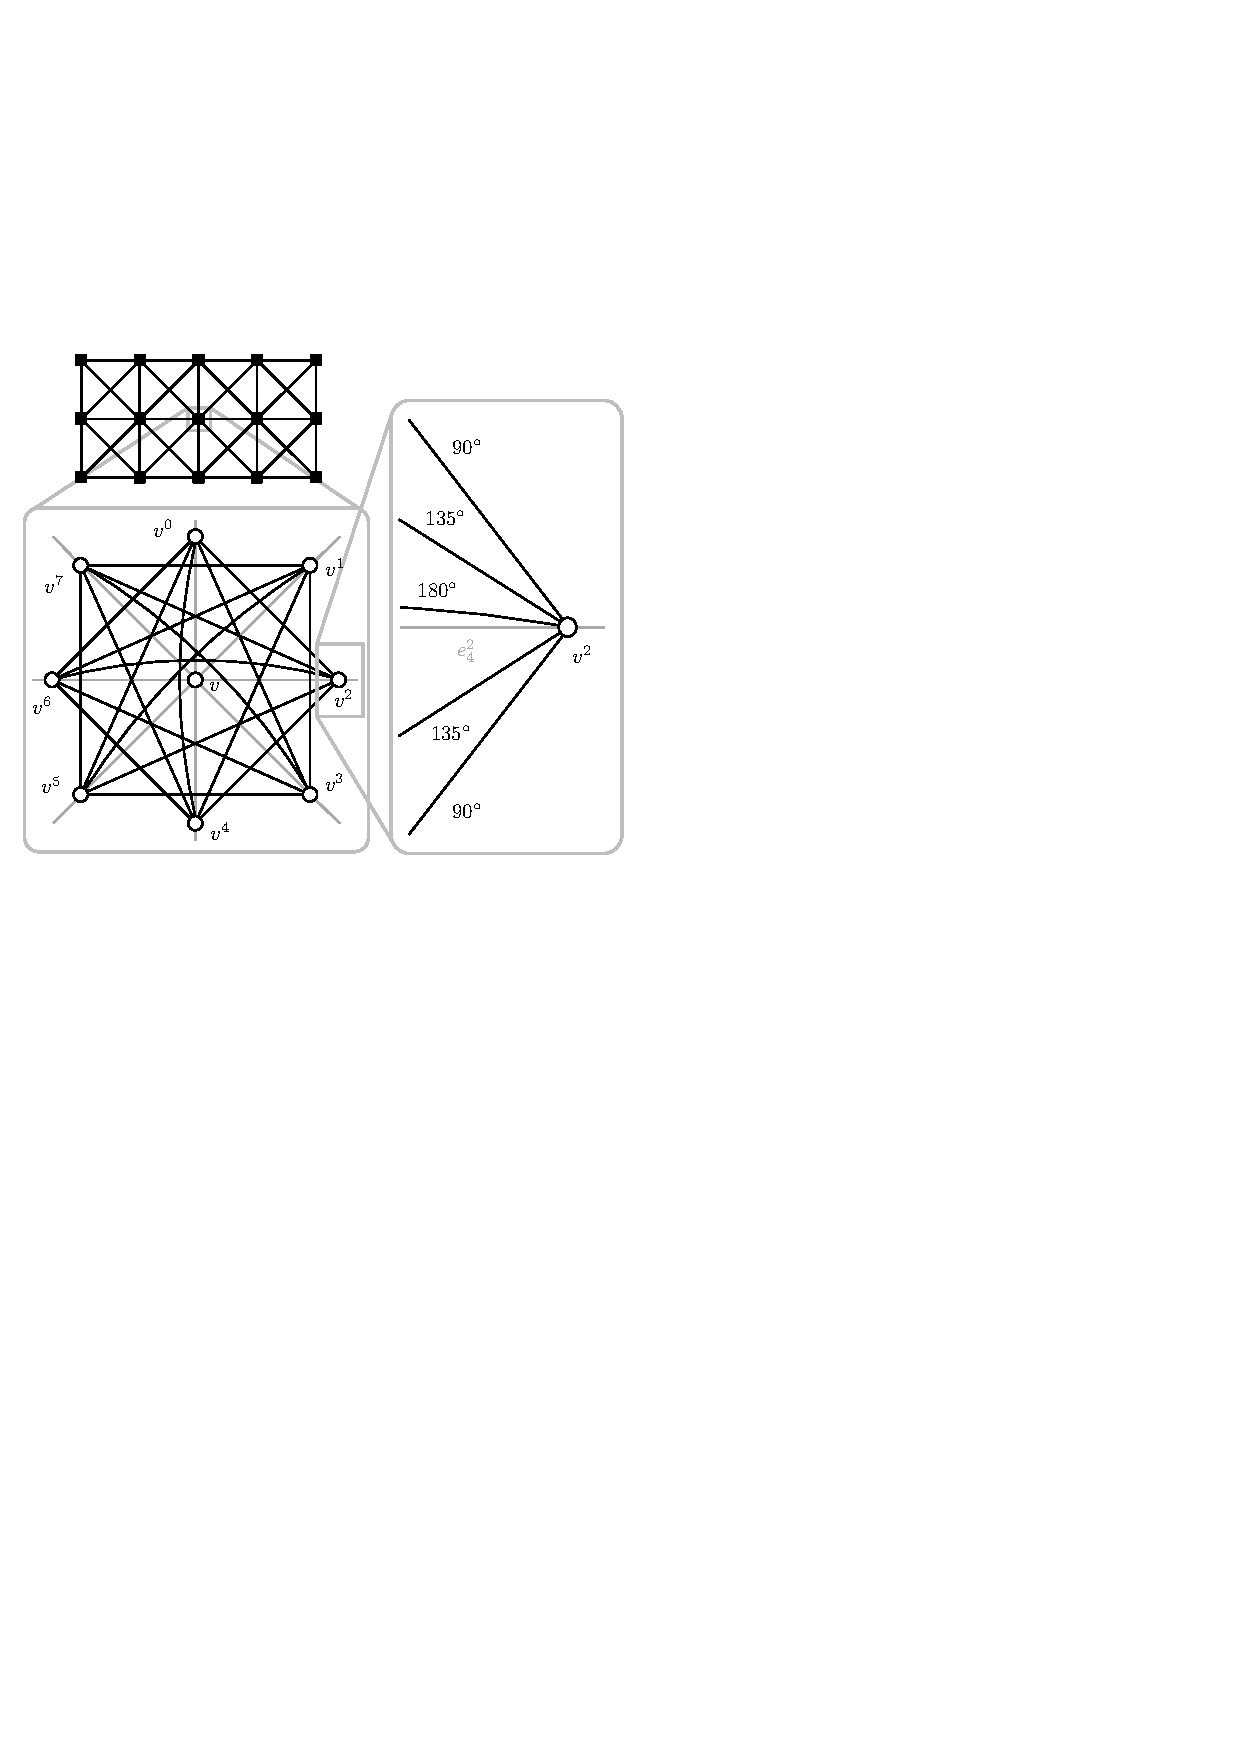
\includegraphics[width=0.45\textwidth]{figures/node.pdf}}}$
	\caption{A $3\times3$ grid graph. Each node $v_i$ has 8 ports $v_i^0 ... v_i^7$ which are connected to $v_i$ by a direct edge. Each port is additionally connected to its $180^{\circ}$, $135^{\circ}$ and $35^{\circ}$ neighbor ports.}
	\label{FIG:gridgraph}
\end{figure}

Following this insight, we introduce a constant $a \geq 0$ and set the port edge costs as follows:
\begin{align}
c_{180} &= a + p_{180} = a \\
c_{135} &= a + p_{135} \\
c_{90} &= a + p_{90} \\
c_{45} &= a + p_{45}.
\end{align}
We choose $a$ in a way such that the following inequalities are fullfilled:
\begin{align}
2a + p_{135} &\geq a + p_{90} \label{CONSTRS:sim90}\\
2a + p_{135} + p_{90} &\geq a + p_{45}\label{CONSTRS:sim45}.
\end{align}
Ineq.~(\ref{CONSTRS:sim90}) ensures that simulating a $90^{\circ}$ pass with two $135^{\circ}$ passes is never cheaper than $c_{90}$. Ineq.~(\ref{CONSTRS:sim45}) ensures that simulating a $45^{\circ}$ pass with a $135^{\circ}$ pass and a $180^{\circ}$ pass is never cheaper than $c_{45}$.

The inequalities are fullfilled for $a = p_{45} - p_{135} \geq 0$, leading to the following port edge costs:

\begin{align}
c_{180} &= p_{45} - p_{135} \\
c_{135} &= p_{45} \\
c_{90} &= p_{45} - p_{135} + p_{90} = c_{180} + p_{90} \\
c_{45} &= 2 p_{45} - p_{135} = c_{180} + c_{135}.
\end{align}

Figure~\ref{FIG:grids}, left provides two example of paths through an octilinear grid graph.

\begin{figure*}[h]
  \centering
	$\vcenter{\hbox{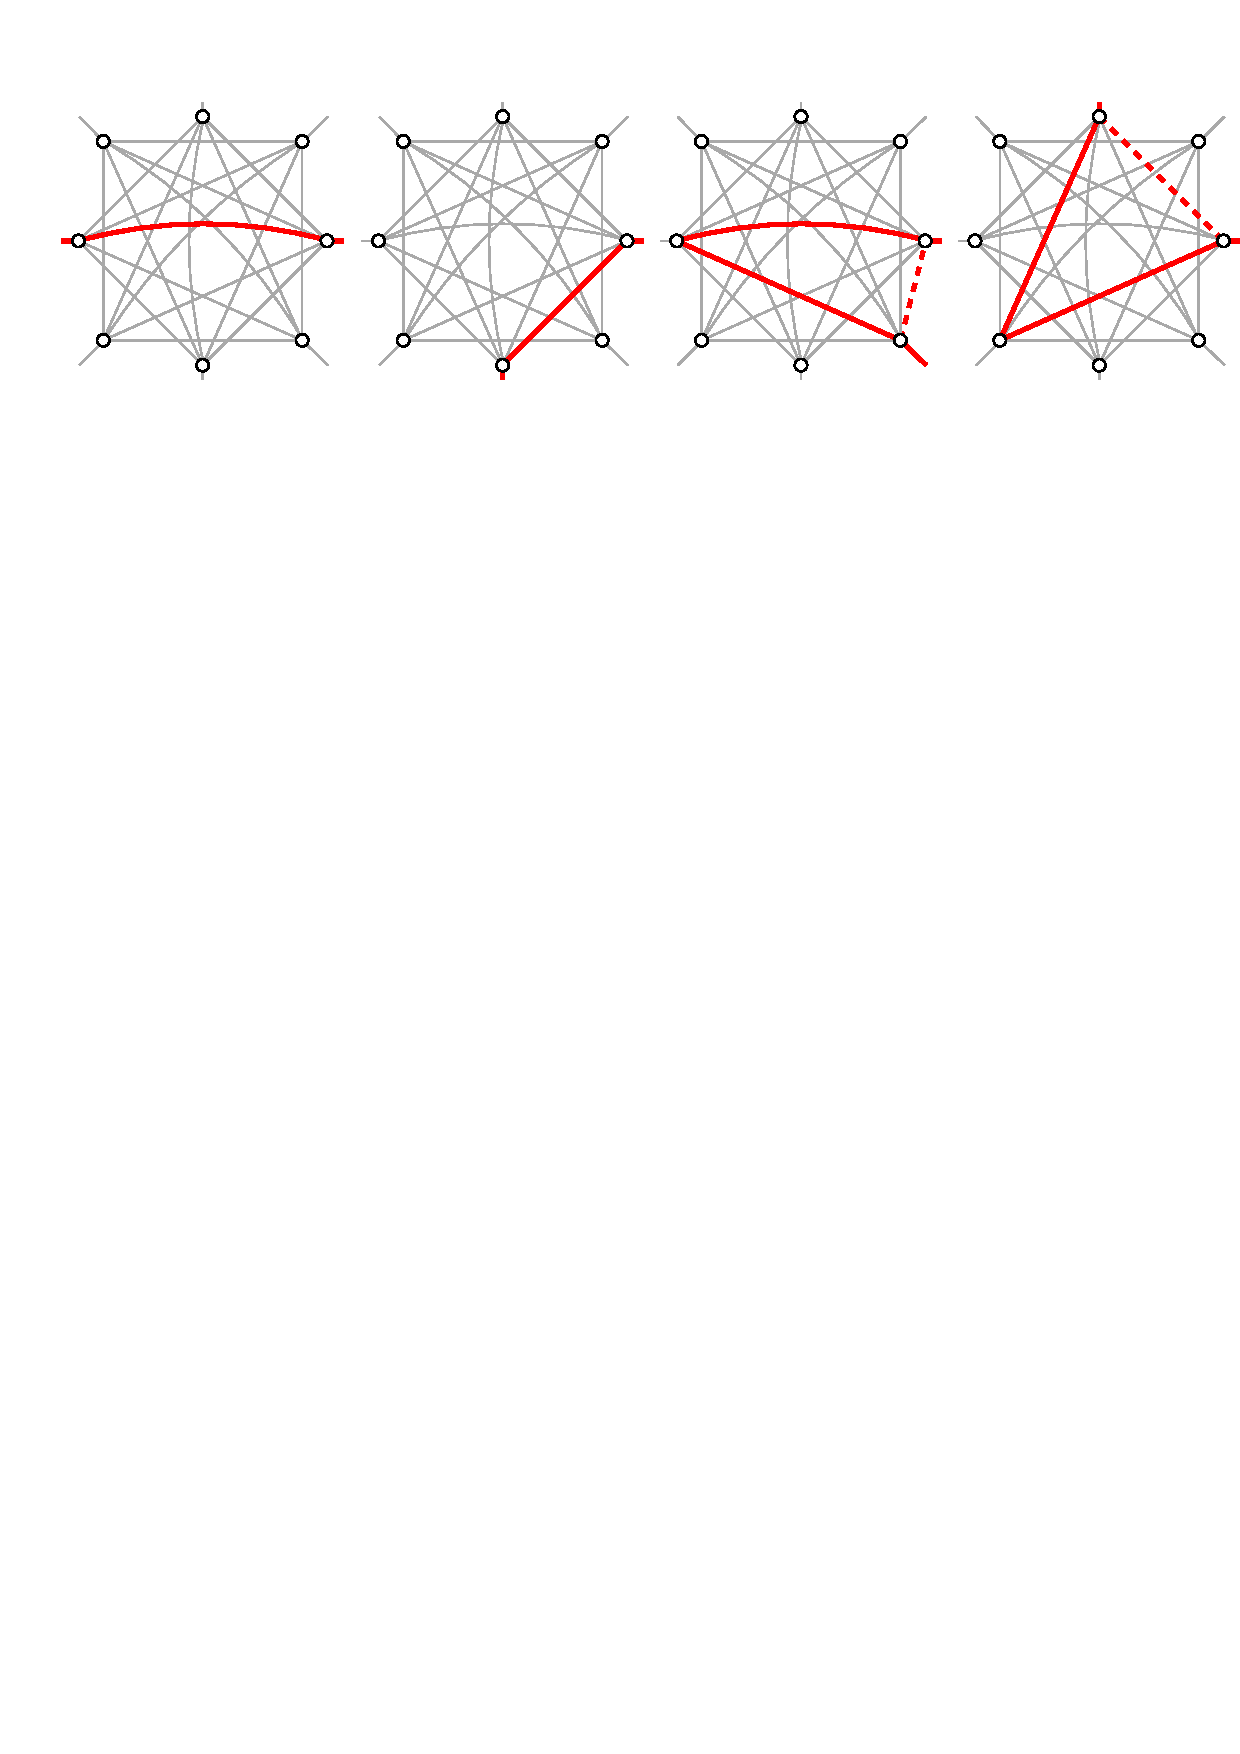
\includegraphics[width=0.9\textwidth]{figures/paths.pdf}}}$
	\caption{1. A $180^{\circ}$ pass through a node $v$. 2. A $90^{\circ}$ pass through $v$. 3. A $45^{\circ}$ pass through $v$ simulated by a $180^{\circ}$ and $135^{\circ}$ pass. 4. A $90^{\circ}$ pass through $v$ simulated by two $135^{\circ}$ passes. }
	\label{FIG:paths}
\end{figure*}

\section{Optimal Solution via Integer Linear Programming}

\subsection{Station Placement}

\subsection{Edge Continuity}

\subsection{Preservement of Embedding}

\subsection{Avoiding Line Bends}

\section{Approximative Solution}

\subsection{Station Placement}

\subsection{Edge Continuity}

\subsection{Preservement of Embedding}

\subsection{Avoiding Line Bends}

\subsection{Optimization via Local Search}

\subsection{Complexity}

\section{Evaluation}

\subsection{Penalty Experiments}

\section{Conclusions}


\balancecolumns
\end{document}
